

Having your project documented with a clean, fresh design is also important. After all, if we put all this work into writing high-quality documentation for our cutting-edge project, it is imperative that the user perceives it as such. Doxygen has all the bells and whistles, but it isn't known for following the latest visual trends. That doesn't mean we'll need a lot of effort to change this, however.

Luckily, a developer known as jothepro created a theme called doxygen-awesome-css that offers a modern, customizable design. It even comes with a dark mode! You can see this in the following screenshot:

\begin{center}
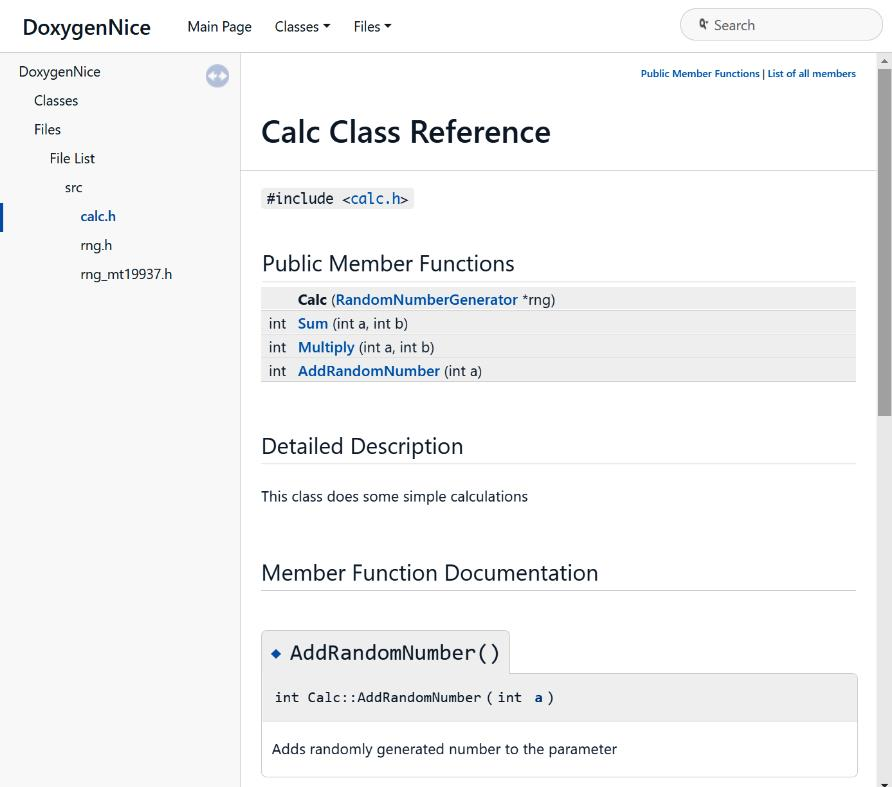
\includegraphics[width=0.8\textwidth]{content/3/chapter10/images/3.jpg}\\
Figure 10.3 – HTML documentation in doxygen-awesome-css theme
\end{center}

The theme doesn't require any additional dependencies and can be easily fetched from its GitHub page at \url{https://github.com/jothepro/doxygen-awesome-css}.

\begin{tcolorbox}[colback=blue!5!white,colframe=blue!75!black,title=Note]
Online sources suggest using multiple applications executed in series to upgrade the experience. One popular approach proposes transforming Doxygen's output with Sphinx using Breathe and Exhale extensions. This process seems a little busy and will pull in a lot of other dependencies (such as Python). I recommend keeping tooling simple where possible. Chances are that not every developer on your project will understand CMake very well, and such a complex process will give them a hard time.
\end{tcolorbox}

We'll go straight to the automated adoption of this theme. Let's see how we can extend our Doxygen.cmake file to use it by adding a new macro, as follows:

\begin{lstlisting}[style=styleCMake]
# chapter-10/02-doxygen-nice/cmake/Doxygen.cmake (fragment)

macro(UseDoxygenAwesomeCss)
	include(FetchContent)
	FetchContent_Declare(doxygen-awesome-css
	GIT_REPOSITORY
		https://github.com/jothepro/doxygen-awesome-css.git
		GIT_TAG
		v1.6.0
	)
	FetchContent_MakeAvailable(doxygen-awesome-css)
	set(DOXYGEN_GENERATE_TREEVIEW YES)
	set(DOXYGEN_HAVE_DOT YES)
	set(DOXYGEN_DOT_IMAGE_FORMAT svg)
	set(DOXYGEN_DOT_TRANSPARENT YES)
	set(DOXYGEN_HTML_EXTRA_STYLESHEET
		${doxygen-awesome-css_SOURCE_DIR}/doxygen-awesome.css)
endmacro()
\end{lstlisting}

We already know all of these commands from previous chapters of the book, but let's reiterate what happens for perfect clarity, as follows:

\begin{itemize}
\item 
doxygen-awesome-css is pulled from Git and made available to the project with the FetchContent module.

\item 
Extra options for Doxygen are configured, as recommended in the theme's README file.

\item 
DOXYGEN\_HTML\_EXTRA\_STYLESHEET configures the path to the theme's .css file. It will be copied to the output directory.
\end{itemize}

As you can imagine, it's best to call this macro in the Doxygen function right before doxygen\_add\_docs(), like this:

\begin{lstlisting}[style=styleCMake]
# chapter-10/02-doxygen-nice/cmake/Doxygen.cmake

function(Doxygen input output)
	...
	UseDoxygenAwesomeCss()
	doxygen_add_docs (...)
endfunction().

macro(UseDoxygenAwesomeCss)
	...
endmacro()
\end{lstlisting}

As a reminder, all variables in macros are set in the scope of the calling function.

We can now enjoy modern style in our generated HTML documentation and share it proudly with the world.















